\textbf{The function $|x-i|$  is analytic for $x\in[-1,1]$. This means it can be analytically continued to an analytic function $f(z)$ in a neighborhood of $[-1,1]$ in the complex z-plane. The formula $|z-i|$ itself does not define an analytic function in any complex neighborhood. Find another formula for $f$ that does, and use it to explain what singularities $f$ has in the complex plane.}
\newline

For a complex function $f(z) = u+vi$ to be analytic, it has to satisfy the Cauchy-Riemann Equations:

\begin{align*}
\frac{\partial u}{\partial x} &= \frac{\partial v}{\partial y},\\
\frac{\partial u}{\partial y} &= -\frac{\partial v}{\partial x}.
\end{align*}
In this case we have that
\begin{align*}
f(z) = |z-i| &= |x+yi-i| \\
&= |x+i(y-1)| \\
&= \sqrt{x^2+(y-1)^2},
\end{align*}
where we have used that $z=x+yi$. Hence we observe that this function is not analytic anywhere since $v=0$ and $u_x$,$u_y$ are not. Therefore we can define 
\begin{align*}
f(z) = f(x) = |x-i| = \sqrt{x^2+1},
\end{align*}
which is analytic within a neighborhood of $x\in [-1,1]$ in the complex plane and has singularities at $z=\pm i$. Hence, like in the previous problem, its Bernstein ellipse is defined by 
\begin{align*}
\rho = 1+\sqrt{2},
\end{align*}
and the exponential convergence is shown in the next figure.
\begin{figure}[H]
\centering
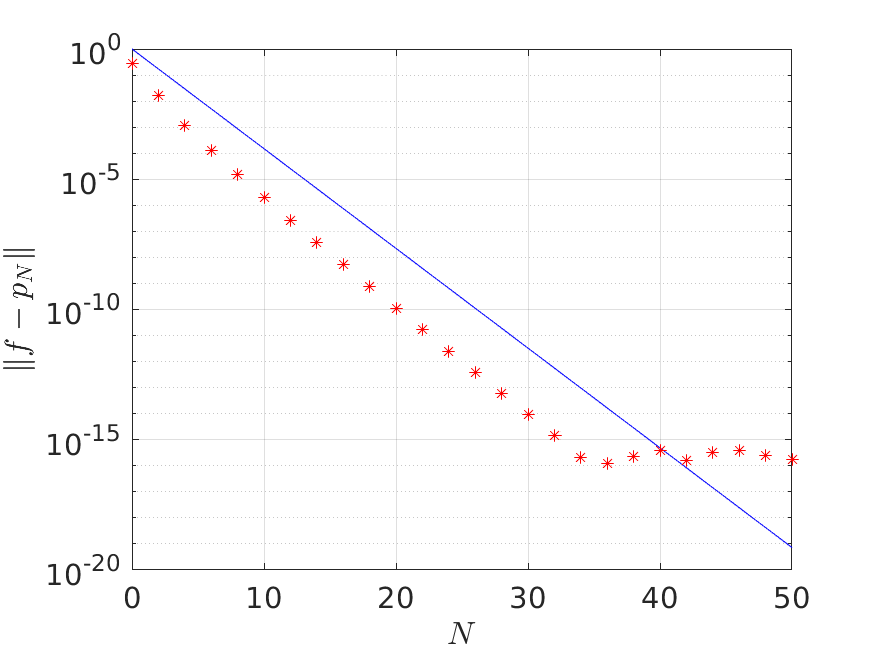
\includegraphics[scale=0.75]{sqrt(x^2+1).png}\caption{Convergence as $n\rightarrow\infty$ of the Chebyshev interpolant to $f(x)=|x-i|$.}
\end{figure}

\subsection*{Matlab code for this section}
\begin{verbatim}
%% Problem 2 - 8.7 ATAP

rho=1+sqrt(2);
orderAcuracy('sqrt(x^2+1)',50,2,rho)
\end{verbatim}